\section{Results}\label{sec:results}

We have improved the REANA platform scheduling performance in order to maximise the scheduling throughput of incoming workflows at the various stages of the workflow life cycle as described in Section~\ref{sec:method}.
A special attention was paid to measure the CPU and Memory usage of the cluster nodes.

Figure~\ref{fig:testnodes} shows a typical snapshot of the status of cluster nodes running the pMSSM workloads.
We have used nodes of the \texttt{m2.xlarge} flavour which consist of 16 GiB of available memory and 8 virtual cores.
One can see the efficient use of cores of the cluster resulting from tuning REANA parameters such as the number of nodes running workflow orchestration tasks, the number of nodes running the pMSSM workflow step jobs themselves, as well as the memory request limits for each ntupling job of the first pMSSM workflow stages.

\begin{figure}
\centering
\footnotesize
\begin{verbatim}
    $ kubectl top nodes
    NAME                                CPU(cores)   CPU%   MEMORY(bytes)   MEMORY%
    reanaatlas1-3slyowp42qex-node-15    7858m        98%    12033Mi         82%
    reanaatlas1-3slyowp42qex-node-16    7848m        98%    12083Mi         83%
    reanaatlas1-3slyowp42qex-node-17    7846m        98%    12210Mi         83%
    reanaatlas1-3slyowp42qex-node-18    7773m        97%    8995Mi          61%
    reanaatlas1-3slyowp42qex-node-19    7864m        98%    11516Mi         79%
    reanaatlas1-3slyowp42qex-node-20    7843m        98%    12177Mi         83%
    reanaatlas1-3slyowp42qex-node-21    7376m        92%    8698Mi          59%
    reanaatlas1-3slyowp42qex-node-22    7817m        97%    11201Mi         77%
    reanaatlas1-3slyowp42qex-node-23    7748m        96%    9978Mi          68%
    reanaatlas1-3slyowp42qex-node-24    7854m        98%    12161Mi         83%
    reanaatlas1-3slyowp42qex-node-25    7868m        98%    12293Mi         84%
    reanaatlas1-3slyowp42qex-node-26    7787m        97%    10991Mi         75%
\end{verbatim}
\caption{An example of the benchmark tests running in the CERN Computer Centre.
The REANA scheduling parameters were optimised to maximise the CPU utilisation and the Memory consumption on the cluster for the typical pMSSM ntupling job parallelism (see Figure~\ref{fig:dag}).
Note the very good efficiency of CPU cores in the above screenshot.}
\label{fig:testnodes}
\end{figure}

Figure~\ref{fig:testresults} shows the results of one of our scalability experiment that consisted of submitting 200 new pMSSM workflows every 10 minutes.
A cluster with 448 cores presented on the left cannot keep up with such a workload: note the increasing scheduling waiting times (plotted in the orange colour) as well as increasing workflow run times (plotted in blue).
The overflow happens because the cluster is allowing more workflows than it can hold.
However, note how the same cluster with 1072 cores presented on the right of the Figure holds the same workload very comfortably.

\begin{figure}
\centering
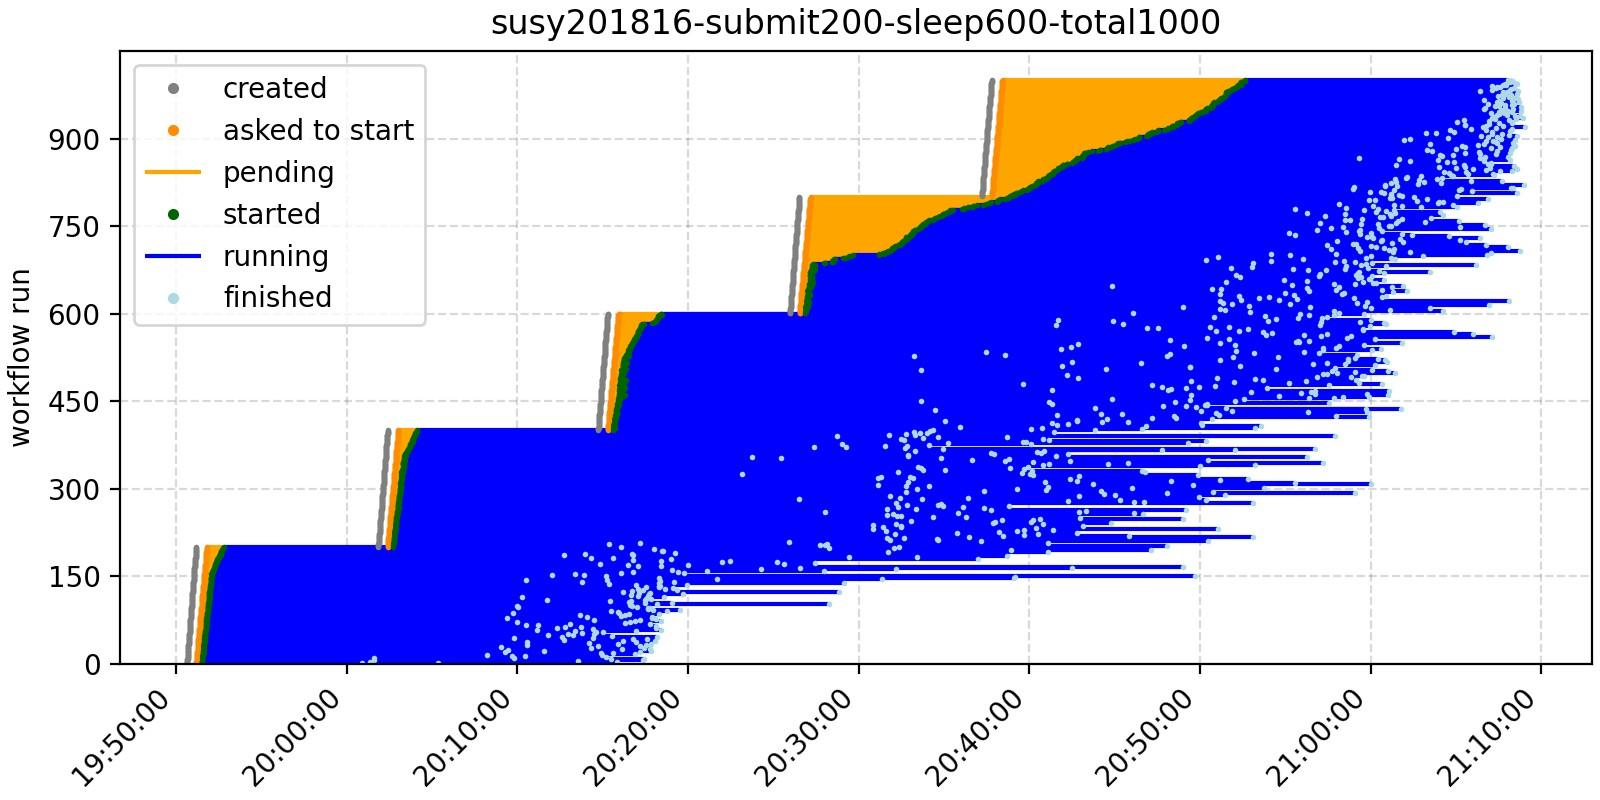
\includegraphics[width=0.45\textwidth]{test-results-1.png}
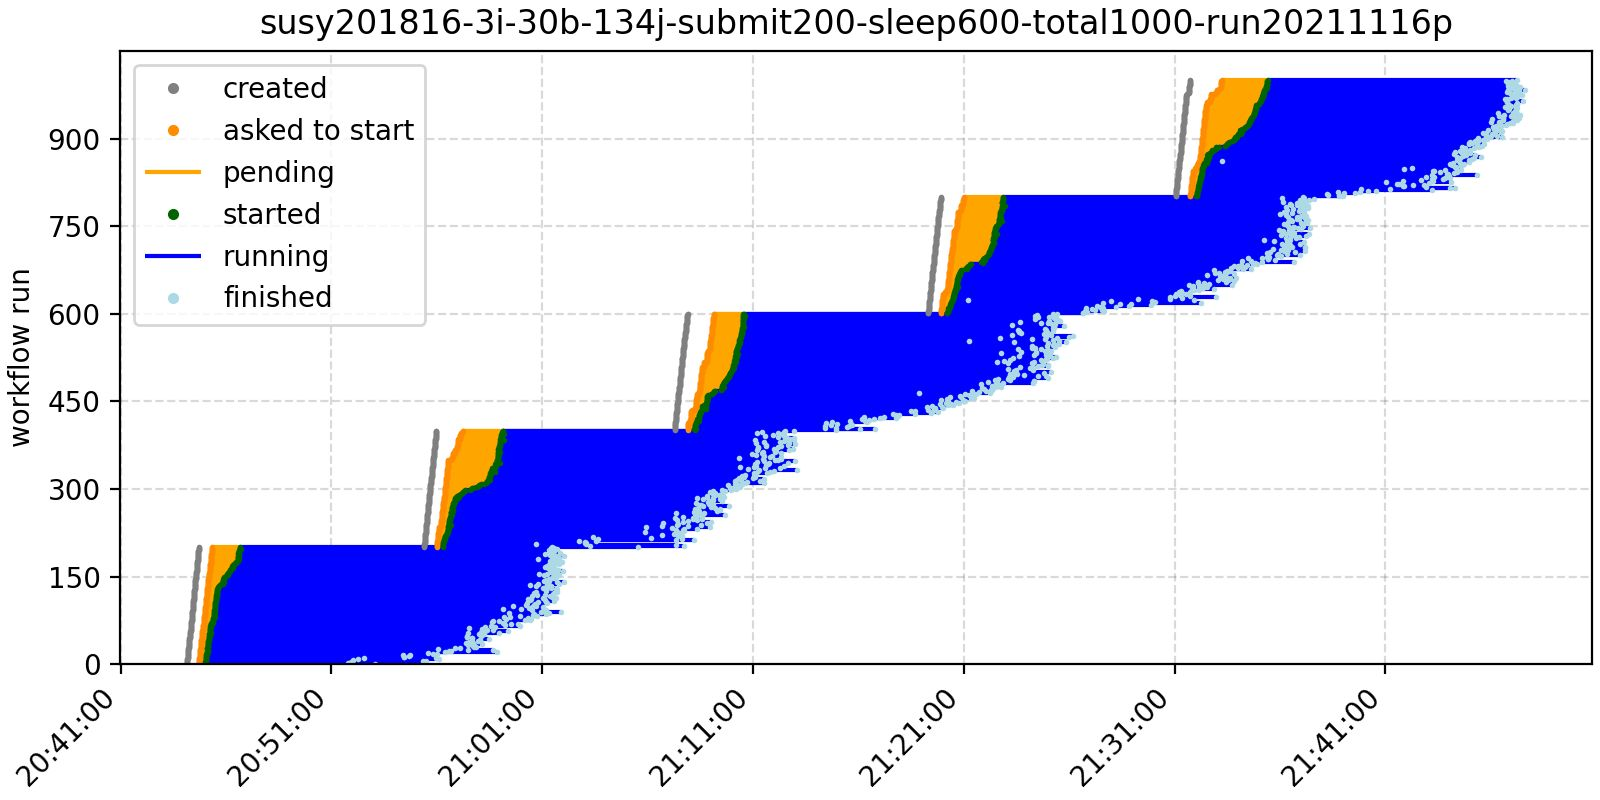
\includegraphics[width=0.45\textwidth]{test-results-2.png}
\caption{A scalability test submitting 200 workflows every 10 minutes.
A cluster with 448 cores (left) cannot keep up with the load.
A cluster with 1072 cores (right) can comfortably hold the incoming workload.}
\label{fig:testresults}
\end{figure}

Figure~\ref{fig:testresultslong} shows the same kind of experiment executed over a longer period of time.
This helped to ensure that the platform can sustain the constantly increasing stream of incoming workloads.

\begin{figure}
\centering
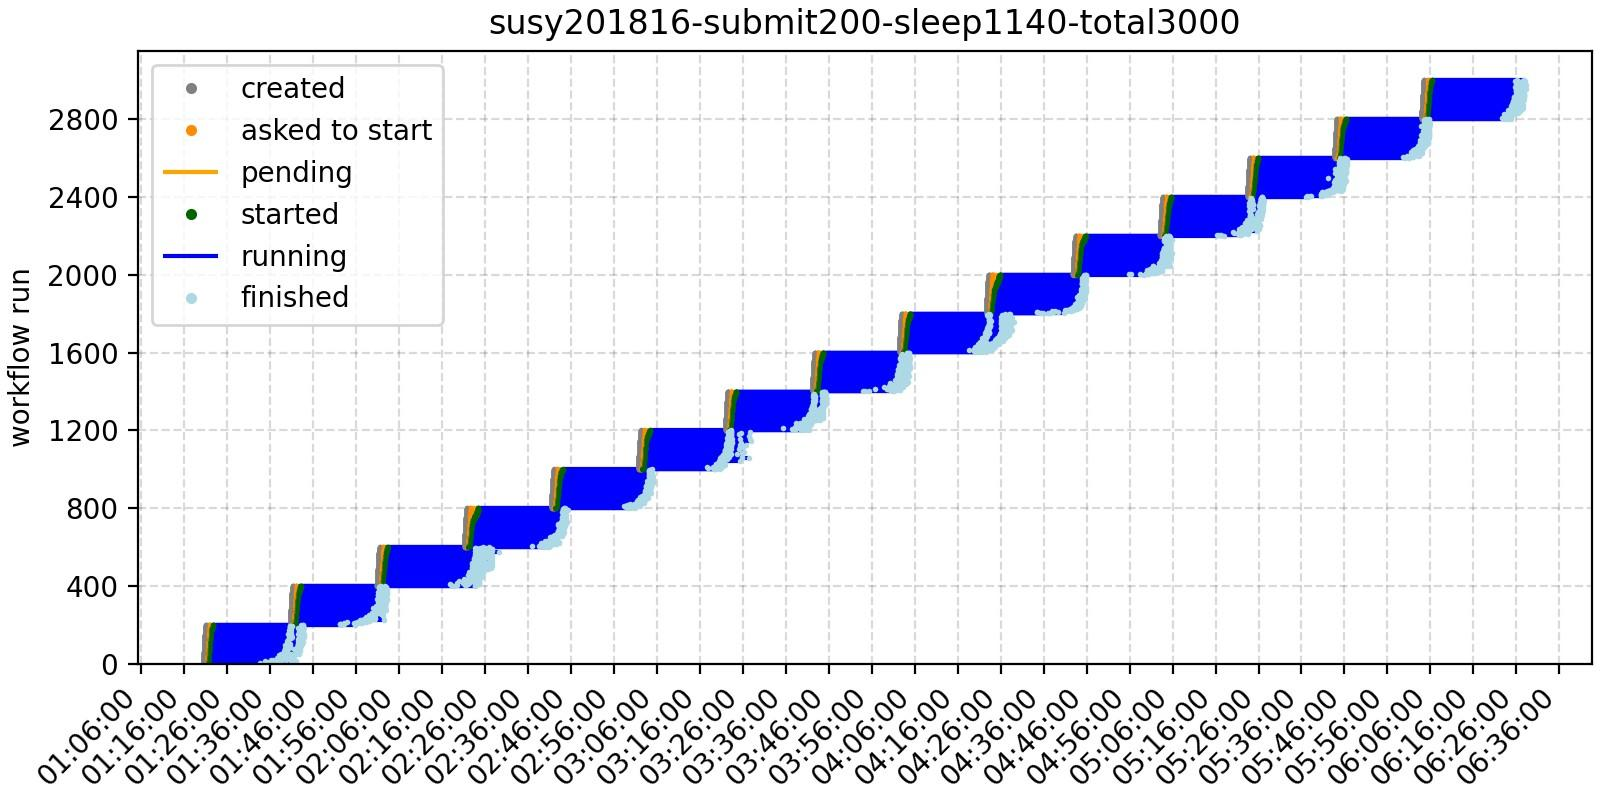
\includegraphics[width=0.9\textwidth]{test-results-3.png}
\caption{The workload burndown throughput rate is sustainable over a long period of time.}
\label{fig:testresultslong}
\end{figure}

We have run several benchmarking experiments in the CERN Computer Centre and, to test the portability, performed a few runs also on the Google Cloud Platform.
This allowed to prove the applicability of the approach on various compute backends, facilitating future reproducibility of containerised workflows irrespective of their original computing environments.
